\documentclass[letterpaper]{article} % DO NOT CHANGE THIS
\usepackage[submission]{aaai2027}  % DO NOT CHANGE THIS
\usepackage[hyphens]{url}  % DO NOT CHANGE THIS
\usepackage{graphicx} % DO NOT CHANGE THIS
\urlstyle{rm} % DO NOT CHANGE THIS
\def\UrlFont{\rm}  % DO NOT CHANGE THIS
\usepackage{natbib}  % DO NOT CHANGE THIS AND DO NOT ADD ANY OPTIONS TO IT
\usepackage{caption} % DO NOT CHANGE THIS AND DO NOT ADD ANY OPTIONS TO IT
\frenchspacing  % DO NOT CHANGE THIS
\usepackage{booktabs}
\usepackage{array}

\pdfinfo{
/TemplateVersion (2027.1)
}

\setcounter{secnumdepth}{0}

\newcommand{\Te}{\ensuremath{T_e}}
\newcommand{\Ge}{\ensuremath{G_e}}
\newcommand{\Ze}{\ensuremath{Z_e}}
\newcommand{\Qe}{\ensuremath{Q_e}}
\newcommand{\Ce}{\ensuremath{C_e}}
\newcommand{\pobs}{\ensuremath{p_{\mathrm{obs}}}}
\newcommand{\prel}{\ensuremath{p_{\mathrm{rel}}}}
\newcommand{\Ssrc}{\ensuremath{S_{\mathrm{src}}}}
\newcommand{\Scomp}{\ensuremath{S_{\mathrm{comp}}}}
\newcommand{\epsscore}{\ensuremath{\epsilon}}
\newcommand{\figbox}[2]{\fbox{\begin{minipage}[t]{#1}\centering\footnotesize #2\end{minipage}}}

\title{Semantic-Geometry Compatibility Learning for Reliable 3D Scene Graph Relations}
\author{Anonymous Submission}
\affiliations{}

\begin{document}

\maketitle

\begin{abstract}
Relation predictors for 3D Scene Graphs return confidence scores for candidate
edges, but confidence is not the same object as reliability. A high score may
reflect a plausible predicate, a source-specific ranking prior, or object-class
co-occurrence, without establishing that the relation is geometrically
compatible with the reconstructed scene. We study this mismatch as a
source-output reliability problem. Rather than applying a universal
semantic-geometry fusion rule, we formulate relation-aware evidence routing:
different relation families call for different evidence routes, including
geometry-only evidence, predicate-geometry compatibility, observability-aware
abstention, or semantic/structural reasoning. We validate the compatibility
route with a factorized score, $\Ce=\mathrm{compatibility}(\Te,\Ge)$, where
$\Te$ encodes predicate and object semantics, $\Ge$ encodes
predicate-independent geometry, and source confidence $\Ze$ is used only after
compatibility has been computed. On VL-SAT and Open3DSG predictions over the
official 3DSSG validation split, compatibility reranking improves the
Recall@K/Violation@K tradeoff on geometry-checkable comparison relations, and a
separate frame-aware scorer supports a qualified left/right lateral result. We
also report route controls and failure analyses: front/behind, support/contact,
observability-heavy, and semantic/structural relations are diagnostic or future
routes, not validated reliability results. The result is a validation-split
reliability study, not a hidden-test benchmark, leaderboard claim, or all-family
solution.
\end{abstract}

\section{Introduction}

3D Scene Graphs represent objects and relations in a scene, and provide a
structured interface for embodied reasoning, scene understanding, and
downstream planning \cite{armeni2019scenegraph,wald2020learning,
wu2021scenegraphfusion}. Modern relation sources can rank candidate relation
edges with high confidence, but such confidence should not be interpreted as a
reliability estimate by default. It may encode a frequent semantic pattern, a
source-specific ranking prior, or object-class co-occurrence rather than
evidence that the predicate is physically compatible with the observed 3D
scene.

This distinction matters for relations whose semantics depend on geometry. For
example, \emph{higher than}, \emph{lower than}, \emph{bigger than}, and
\emph{smaller than} require predicate-specific interpretation of geometric
evidence. In contrast, \emph{close by} may be nearly geometry-decidable, while
\emph{attached to}, \emph{inside}, and \emph{cover} may require observability
or visual/mesh evidence before a reliable decision can be made. Relations such
as \emph{part of} or identity/symmetry predicates are better viewed as
semantic or structural routes. A single fixed fusion of source confidence and
geometry is therefore too coarse.

We therefore treat reliable 3D relation estimation as an evidence-routing
problem. The proposed formulation separates semantic content, source
confidence, geometry evidence, compatibility, and observability. Its validated
mechanism is predicate-geometry compatibility:
$\Ce=\mathrm{compatibility}(\Te,\Ge)$ is computed without source confidence
$\Ze$, and $\Ze$ enters only when reranking a source prediction list. This
separation is essential. If compatibility can copy source score or rank, it no
longer tests whether predicate semantics and geometry support each other.

\paragraph{Claim boundary.}
The claim is deliberately bounded. We do not solve reliable 3D relation
estimation across all relation families. We propose relation-aware evidence
routing and validate its predicate-geometry compatibility route on
geometry-checkable comparison relations. We also report a qualified left/right
lateral result. We do not claim an official 3DSSG hidden-test result,
leaderboard performance, a support/contact reliability result, a calibrated
$\pobs/\prel$ benchmark, or a completed all-family reliability system.

\paragraph{Contributions.}
We make four contributions. First, we formulate 3D Scene Graph relation
reliability as relation-aware evidence routing rather than universal confidence
fusion. Second, we introduce a factorized edge representation that separates
$\Te$, $\Ge$, $\Ze$, $\Qe$, $\Ce$, $\pobs$, and $\prel$, and enforce that
$\Ce$ is computed before source confidence enters final reranking. Third, we
evaluate a source-output reranking score,
$\Scomp(e)=\mathrm{norm}(\Ze)\cdot\Ce$, on VL-SAT and Open3DSG validation
predictions. Fourth, we report controls, ablations, and boundary routes that
specify where the current evidence is sufficient and where richer
relation-specific evidence is still required.

\begin{figure*}[t]
\centering
\setlength{\fboxsep}{4pt}
\begin{tabular}{ccccc}
\figbox{0.18\textwidth}{\textbf{Relation source}\\VL-SAT/Open3DSG\\candidate edge $e=(s,p,o)$\\source score/rank $\Ze$}
&
$\rightarrow$
&
\figbox{0.22\textwidth}{\textbf{Model-safe evidence}\\semantic content $\Te$\\predicate-independent geometry $\Ge$\\\emph{no source score/rank}}
&
$\rightarrow$
&
\figbox{0.20\textwidth}{\textbf{Validated mechanism}\\$\Ce=f_{\theta}(\Te,\Ge)$\\predicate--geometry compatibility}
\\[3pt]
&&&&\\[-8pt]
\multicolumn{5}{c}{$\downarrow$ source confidence enters only after compatibility is computed}\\[-1pt]
\multicolumn{5}{c}{\figbox{0.68\textwidth}{\textbf{Validation reranking path}\\$\Scomp(e)=\mathrm{norm}(\Ze)\cdot \Ce$ compared with $\Ssrc(e)=\Ze$ using Recall@K and custom Violation@K on the official 3DSSG validation split.}}
\end{tabular}
\vspace{4pt}

\begin{tabular}{p{0.16\textwidth}p{0.17\textwidth}p{0.17\textwidth}p{0.17\textwidth}p{0.17\textwidth}}
\toprule
\textbf{Validated} & \textbf{Qualified} & \textbf{Diagnostic} & \textbf{Future} & \textbf{Excluded claims} \\
\midrule
higher/lower; bigger/smaller & left/right lateral & close by geometry-only; front/behind; support/contact & attachment; containment; semantic/structural; calibrated $\pobs/\prel$ & hidden-test benchmark; all-family reliability; support/contact reliability \\
\bottomrule
\end{tabular}
\caption{Compatibility reranking and route boundary. The validated path computes
predicate-geometry compatibility $\Ce$ from $\Te$ and $\Ge$, then combines it
with source confidence $\Ze$ only for final source reranking. The bottom row
separates validated, qualified, diagnostic, and future routes so the framework
is not read as an all-family reliability system.}
\label{fig:score-flow}
\end{figure*}

\section{Related Work}

\paragraph{Scene graph foundations and source predictors.}
Scene graphs have long been used as explicit object-relation representations
for retrieval and visual reasoning \cite{johnson2015image}, with Visual Genome
providing dense object, attribute, and relationship annotations
\cite{krishna2017visualgenome}. 2D SGG methods model graph context, message
passing, object-predicate regularities, and dataset bias
\cite{xu2017iterative,zellers2018neuralmotifs,yang2018graphrcnn,
tang2020unbiased}. 3D Scene Graphs extend this idea to semantics grounded in
3D space and camera structure \cite{armeni2019scenegraph}. 3DSSG and 3RScan
then made relation prediction from changing indoor reconstructions a standard
benchmark setting \cite{wald2019rio,wald2020learning}.

\paragraph{3D SGG, online graphs, and open vocabulary.}
Follow-up systems predict or update 3D scene graphs from point clouds and
RGB-D/RGB streams, including incremental RGB-D graph construction, RGB-only
incremental prediction, online graph generation, and knowledge-guided point
cloud prediction \cite{wu2021scenegraphfusion,wu2023rgbsgg,hou2025fross,
zhang2021knowledge3d,qiu2023kg3dsg}. VL-SAT uses visual-linguistic semantics
to assist 3DSSG prediction \cite{wang2023vlsat}. Open3DSG and ConceptGraphs
move toward open-vocabulary 3D graph sources
\cite{koch2024open3dsg,gu2024conceptgraphs}. We use VL-SAT and Open3DSG as
source candidate generators; the proposed method is a reliability layer over
their outputs, not a replacement predictor.

\paragraph{Visual-geometric evidence and witnesses.}
Point-cloud encoders such as PointNet and PointNet++ motivate learned 3D
geometry representations \cite{qi2017pointnet,qi2017pointnetpp}, and recent
3D SGG work increasingly uses geometric or visual-geometric evidence. RelWitness
explicitly frames relation verification around visual-geometric cues that make
a relation observable \cite{nguyen2026relwitness}. This directly rules out a
weak novelty claim that merely ``adds geometry.'' Our approach therefore
separates source confidence $\Ze$, semantic content $\Te$,
predicate-independent geometry evidence $\Ge$, compatibility $\Ce$, and
observability $\Qe$, then specifies which factors are appropriate for each
relation route.

\paragraph{Reliability, uncertainty, and conditional evidence use.}
Calibration studies whether model confidence estimates correctness likelihood
\cite{guo2017calibration,nixon2019calibration}. Predictive uncertainty and
selective prediction study when a model should avoid overconfident decisions
\cite{lakshminarayanan2017deepensembles,geifman2017selective,
geifman2019selectivenet}. Conditional computation, missing-modality learning,
and gated fusion show how inputs can be routed, combined, or abstained under
different evidence conditions \cite{shazeer2017moe,wu2018mvae,shi2019mmvae,
perez2018film,arevalo2017gmu}. We borrow the principle of conditional evidence
use but specialize it to 3D relation reliability: the route
assignment determines whether geometry-only evidence, predicate-geometry
compatibility, observability-aware abstention, or semantic/structural reasoning
is appropriate.

\section{Problem Definition}

Let $e=(s,p,o)$ be a candidate relation edge with subject object $s$,
predicate $p$, and object $o$. A source model provides a confidence and rank
for $e$. We distinguish the following factors:

\begin{itemize}
\item $\Te$: predicate, relation-family, and subject/object semantic content.
\item $\Ge$: predicate-independent geometry evidence for the object pair.
\item $\Ze$: source confidence, rank, and source-specific score information.
\item $\Qe$: observability and evidence-quality information.
\item $\Ce$: predicate-geometry compatibility computed from $\Te$ and $\Ge$.
\item $\pobs$: probability that available evidence is sufficient to judge the
relation.
\item $\prel$: relation reliability probability under sufficient evidence.
\end{itemize}

The validated compatibility route first fits a source-agnostic raw score
\[
C_e^{\mathrm{raw}} = f_{\theta}(\Te,\Ge),
\]
where $\Ze$ is excluded from $f_{\theta}$. We then apply label-free min--max
normalization per source-family candidate pool and rerank with
\[
\Ce=\mathrm{norm}_{\mathrm{source,family}}(C_e^{\mathrm{raw}}),
\]
\[
\Scomp(e)=\mathrm{norm}_{\mathrm{source}}(\Ze)\cdot\Ce.
\]
The source baseline is $\Ssrc(e)=\Ze$. The paper evaluates the Recall@K and
Violation@K tradeoff after reranking. Recall@K measures GT relation recovery
under the validation mapping. Violation@K is a custom geometry-consistency
metric that measures how often selected edges violate route-specific geometric
checks. It is not an official 3DSSG benchmark metric.

\paragraph{Route assignment protocol.}
The route taxonomy is part of the method rather than a post-hoc result table.
For each relation family we ask six questions: (1) can metric geometry alone
decide the relation, (2) does the predicate change how geometry should be
interpreted, (3) is a reference frame required, (4) is contact or pose evidence
required, (5) is visual/mesh observability required before a decision is
possible, and (6) is the relation mainly semantic, structural, identity, or
symmetry reasoning? These questions determine whether the candidate enters a
geometry-only route, a predicate-geometry compatibility route, a frame-aware
route, a hard contact/pose route, an observability-aware route, or a
semantic/structural boundary route. Only the comparison compatibility route and
the qualified left/right lateral route are treated as quantitative validation
routes in this manuscript.

\begin{table*}[t]
\centering
\small
\setlength{\tabcolsep}{4pt}
\begin{tabular}{p{0.18\textwidth}p{0.23\textwidth}p{0.18\textwidth}p{0.29\textwidth}}
\toprule
Route & Relation types & Manuscript role & Evidence requirement \\
\midrule
Predicate--geometry compatibility & higher/lower, bigger/smaller & validated route & Predicate changes how the same geometry evidence should be interpreted. \\
Bounded lateral compatibility & left/right & qualified validation route & Frame-aware direction reduces violations, but one source loses some recall. \\
Geometry-only compatibility & close by & control route & Distance evidence is sufficient, so complex compatibility is unnecessary. \\
Frame/depth ambiguity & front/behind & failure route & Reference frame and depth ambiguity cause large recall losses. \\
Hard contact/pose & standing on, lying on, supported by & diagnostic failure analysis & Contact, pose, mesh, and subtype evidence are required before a reliability claim. \\
Observability-heavy & attached to, hanging on, inside, cover & future validation route & The first question is whether required visual/mesh evidence is observable. \\
Semantic/structural & part of, belonging to, identity/symmetry & scope boundary & Reliability depends on structural or identity evidence beyond scalar geometry. \\
\bottomrule
\end{tabular}
\caption{Route assignment protocol and claim boundary. The table is a
method-level evidence map, not a family-level performance table. Each row is
assigned by the evidence required to judge relation reliability.}
\label{tab:route-taxonomy}
\end{table*}

\section{Method}

\paragraph{Leakage-controlled views.}
We use three views of each candidate edge. The model-safe view contains
$\Te$ and $\Ge$ for compatibility scoring. The source-rank view contains
$\Ze$ for final reranking. The hidden metric manifest contains GT labels,
violation labels, construction fields, and audit-only metadata. Hidden fields
are never model inputs.

\paragraph{Compatibility scoring.}
The raw compatibility model is source-agnostic. It asks whether the predicate
semantics in $\Te$ are compatible with the geometry evidence in $\Ge$;
$\Ce$ denotes its label-free source-family normalization used for reranking.
For comparison relations, $\Ge$ contains signed or
route-normalized geometric evidence such as vertical order or size difference,
while $\Te$ identifies which predicate interpretation is required. The score
is not allowed to use source score or rank.

\paragraph{Score conditions and controls.}
The source-only baseline is $\Ssrc(e)=\Ze$. The primary compatibility reranking
score is $\Scomp(e)=\mathrm{norm}(\Ze)\cdot\Ce$. A geometry-only ablation tests
whether route-aware geometry alone explains the result. A plain $\Te/\Ge$
concatenation ablation tests whether generic fusion is sufficient. Additional
controls include compatibility-only diagnostics, shuffled $\Ce$, shuffled
geometry, and wrong-predicate $\Te$ controls. These
rows test whether the score depends on matched predicate and geometry rather
than source rank, geometry alone, or construction leakage. We treat these
controls as counterfactual identifiability checks: a valid $\Ce$ should change
under wrong predicate, shuffled geometry, wrong-pair geometry, or direction
swap interventions.

\paragraph{Source reranking.}
After $\Ce$ is computed, source confidence is combined only for reranking:
\[
\Scomp(e)=\mathrm{norm}(\Ze)\cdot\Ce.
\]
This makes the method a source-output reliability layer rather than a
replacement for VL-SAT or Open3DSG. The design tests whether matched predicate-geometry
compatibility can improve source ranking while reducing geometry violations.

\paragraph{Risk-aware score interpretation.}
The product score is not used as an arbitrary heuristic. In log space it is the
$\lambda=1$ case of a risk-aware reranking utility:
\[
\log \Scomp(e)=\log \mathrm{norm}(\Ze)-\lambda r(e),
\quad r(e)=-\log \Ce.
\]
We use $\lambda=1$ as a parameter-free product form to avoid tuning a risk
weight on validation labels. Equivalently, $\Ze$ and $\Ce$ can be read as two
evidence experts:
\[
P_{\mathrm{source}}(\cdot\mid \Ze)\,
P_{\mathrm{comp}}(\cdot\mid \Te,\Ge).
\]
This interpretation depends on the leakage boundary above: $\Ce$ is computed
without $\Ze$, and therefore cannot simply copy the source rank.

\paragraph{Score normalization.}
The main $\mathrm{norm}(\Ze)$ uses label-free per-source min--max
normalization over the validation candidate pool, and $\Ce$ is the raw logistic
compatibility probability normalized per source-family candidate pool. No validation label,
Violation@K label, or hidden metric field is used to define these bounds. For
the log interpretation only, both terms are clamped to $[\epsscore,1]$ with
$\epsscore=10^{-6}$; the implemented product score uses the same clipped
normalized terms.

\paragraph{Selective decision layer.}
The framework includes $\Qe$, $\pobs$, and $\prel$ for observability-aware
selective decisions. In this scoped manuscript, they remain framework
components and stress tests; calibrated selective reliability is left for
future validation.

\section{Experiments}

\paragraph{Data and sources.}
All reported quantitative results in this manuscript use the official 3DSSG
validation split. We use validation because public 3DSSG-style relation labels
and source predictions are available for reproducible comparison, whereas this
submission does not use a hidden test server. We rerank validation predictions
from VL-SAT and Open3DSG. Open3DSG is treated as an open-vocabulary relation
source, but quantitative Recall@K is computed after closed-vocabulary 3DSSG
mapping. Thus the source may be open vocabulary, but the reported Recall table
is a closed-vocabulary validation-level evaluation.

\paragraph{Routes and metrics.}
The primary evaluated route consists of geometry-checkable comparison relations:
higher than, lower than, bigger than, and smaller than. The qualified lateral
route consists of left and right. Front/behind is not pooled with left/right;
it is reported as a frame/depth ambiguity failure case. The main metrics are
Recall@K and Violation@K over $K\in\{5,10,20,50,100\}$. Violation@K is a custom
geometry-consistency metric, not an official benchmark metric. Bootstrap
confidence intervals are computed for the reported $\Scomp-\Ssrc$ deltas and
for selected ablation deltas.

\paragraph{Claim boundary.}
The experiment is a validation-split study. It does not use hidden-test labels
or claim leaderboard performance, full relative-horizontal success, or
all-family 3D relation reliability. Support/contact and observability-heavy
relations are used to identify hard routes and future evidence requirements.

\section{Results}

\subsection{Main Comparison Route}

Figure~\ref{fig:main-comparison} reports validation-split source reranking on
the core comparison route. \Scomp{} improves Recall@K while
substantially reducing Violation@K for K = 10, 20, and 50. K = 5 is not a
strong recall claim because its Recall confidence interval includes zero. K =
100 is not central because the candidate list is close to saturation. The main
evidence is the mid-K tradeoff: more GT relations are retained while fewer
geometry-inconsistent edges enter the selected top-K set.

\begin{figure}[t]
\centering
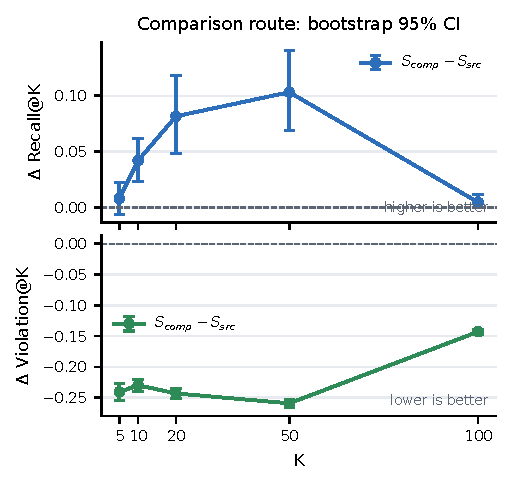
\includegraphics[width=\columnwidth]{figures/comparison_tradeoff_ci.pdf}
\caption{Validation-split source reranking for the
geometry-checkable comparison route only (higher/lower and bigger/smaller).
Values are $\Scomp-\Ssrc$ deltas with bootstrap 95\% intervals over validation
candidate units; exact values are reported in Supplementary Table~S1. This is
not a hidden-test result, all-family
benchmark, or leaderboard claim.}
\label{fig:main-comparison}
\end{figure}

At K = 20, the absolute comparison-route values are $\Ssrc$ Recall = 0.6429
and Violation = 0.3436 versus $\Scomp$ Recall = 0.7245 and Violation = 0.1005.

\subsection{Ablation Summary}

At K = 20, compatibility reranking outperforms source-only, route-aware geometry-only, and plain
$\Te/\Ge$ concatenation. The selected confidence intervals support that the
gain is not reducible to geometry-only reranking or plain concatenation. If
the effect were only a geometry rule, the geometry-only ablation would match
the primary score. If it were only generic feature fusion, the concat ablation
would match the primary score. The observed gap supports the
specific role of matched predicate-geometry compatibility.

\begin{table}[t]
\centering
\scriptsize
\setlength{\tabcolsep}{3pt}
\begin{tabular}{lrrp{0.22\linewidth}}
\toprule
Score & R@20 & V@20 & Role \\
\midrule
Source & 0.6429 & 0.3436 & baseline \\
G-only & 0.6463 & 0.3275 & geometry ablation \\
Concat & 0.6293 & 0.3308 & fusion ablation \\
Compat. & 0.7245 & 0.1005 & primary \\
\bottomrule
\end{tabular}
\caption{Mechanism-check ablations for the comparison route. The rows are not
standalone benchmark systems. They test whether compatibility reranking is explained by source
ranking, geometry-only filtering, or generic concatenation.}
\label{tab:ablations}
\end{table}

Selected bootstrap CI deltas at K = 20 are:
$\Delta$(Compat.-G-only) Recall@20 = [0.0475, 0.1103] and Violation@20 =
[-0.2348, -0.2193]; $\Delta$(Compat.-Concat) Recall@20 = [0.0647, 0.1312] and
Violation@20 = [-0.2389, -0.2222].

\subsection{Qualified Left/Right Route}

Left/right is included as a qualified lateral route, not as full
relative-horizontal success. Open3DSG left/right gains are strong, while
VL-SAT left/right trades small recall losses for lower violation. This supports
including left/right as a qualified validation route while excluding a full
left/right/front/behind reliability claim.

\begin{table}[t]
\centering
\scriptsize
\setlength{\tabcolsep}{2.5pt}
\begin{tabular}{llrrrr}
\toprule
Source & K & $\Delta$R & R CI & $\Delta$V & V CI \\
\midrule
Open3DSG & 20 & 0.269 & [0.235, 0.303] & -0.466 & [-0.479, -0.454] \\
Open3DSG & 50 & 0.378 & [0.335, 0.419] & -0.367 & [-0.382, -0.351] \\
VL-SAT & 20 & -0.043 & [-0.057, -0.030] & -0.100 & [-0.111, -0.089] \\
VL-SAT & 50 & -0.021 & [-0.033, -0.012] & -0.124 & [-0.134, -0.116] \\
\bottomrule
\end{tabular}
\caption{Selected left/right qualified lateral results using the frozen
frame-aware scorer. The route reduces violation risk, but the VL-SAT recall
tradeoff prevents a uniform-improvement claim.}
\label{tab:left-right}
\end{table}

\subsection{Failure and Boundary Routes}

Front/behind is kept as frame/depth ambiguity. In selected cells, violation is
reduced but recall losses are large, e.g., Open3DSG K = 50 has
$\Delta$Recall = -0.1704 and $\Delta$Violation = -0.3592, while VL-SAT K = 20
has $\Delta$Recall = -0.2031 and $\Delta$Violation = -0.2731.
Support/contact does not provide a reliability result under the current
evidence. The latest proxy-target repair yields only 35 accept and 347 reject
binary rows, so a reject-only classifier already reaches 0.908 accuracy.
Moreover, the geometry-rule construction state recovers the binary target with
1.0 leave-one-out accuracy and macro recall. This is target circularity, not
evidence that support/contact reliability has been learned; metric reruns and
solved-route wording are therefore blocked.

\begin{table}[t]
\centering
\scriptsize
\setlength{\tabcolsep}{3pt}
\begin{tabular}{p{0.22\linewidth}p{0.31\linewidth}p{0.31\linewidth}}
\toprule
Route & Observed failure & Paper interpretation \\
\midrule
front/behind & violation decreases, but recall losses are large & reference-frame/depth evidence is required before promotion \\
support/contact repair & 35/382 positives; 0.908 majority; geometry-rule state recovers target at 1.0/1.0 & circular proxy target; no metric or solved-route claim \\
supported by & broad label mixes support existence and subtype & relabel-or-abstain boundary case requiring independent labels \\
attach/contain & scalar geometry cannot decide observability & future visual/mesh $\Qe$ route \\
\bottomrule
\end{tabular}
\caption{Failure taxonomy used to bound the scoped claim. These rows motivate
the broader relation-aware framework but are not counted as validated routes.}
\label{tab:failure-taxonomy}
\end{table}

\begin{table}[t]
\centering
\scriptsize
\setlength{\tabcolsep}{3pt}
\begin{tabular}{p{0.23\linewidth}p{0.34\linewidth}p{0.27\linewidth}}
\toprule
Example pattern & Row-level evidence type & Interpretation \\
\midrule
comparison edge with high source score but wrong sign & edge is reranked down when $\Ce$ disagrees with vertical or size evidence & source confidence is not relation reliability \\
left/right lateral correction & frame-aware score lowers violation while preserving Open3DSG recall & lateral route is useful but source-dependent \\
front/behind candidate & violation can fall while recall drops sharply & depth/reference-frame ambiguity blocks promotion \\
close-by proximity row & normalized distance is already sufficient in source-wide diagnostics & geometry-only route, not a predicate-geometry interaction claim \\
support/contact proxy rows & accept/reject labels are sparse and exactly recoverable from the construction rule & target independence must precede richer pose/contact modeling \\
\bottomrule
\end{tabular}
\caption{Qualitative row-pattern examples used for failure analysis. They
explain route behavior and reviewer-risk boundaries; they are not additional
validated-route metrics.}
\label{tab:qualitative-patterns}
\end{table}

\section{Discussion and Limitations}

\paragraph{Validated scope.}
The validated quantitative mechanism is predicate-geometry compatibility on
comparison relations, plus a qualified left/right lateral route. This is enough
to support the design claim that source confidence and fixed fusion are
insufficient for geometry-checkable relation reliability, but it is not enough
to establish reliable 3D relations across all families.

\paragraph{Route-aware framework boundary.}
The framework remains broader than the validated mechanism. Close by is a
geometry-only control route, front/behind exposes reference-frame and depth
ambiguity, support/contact exposes the need for richer contact and pose
evidence but its current proxy target is circular, observability-heavy relations require visual/mesh evidence and
selective decisions, and semantic/structural relations may require non-geometry
evidence. These routes are part of the framework boundary, but not validated
reliability routes in this manuscript.

\paragraph{Validation split.}
The reported tables are validation-level evaluations on the official 3DSSG
validation split. They should not be described as hidden-test or leaderboard
results.

\paragraph{Normalization and calibration.}
The main compatibility reranking score uses frozen label-free candidate-pool normalization. We
report normalization sensitivity rather than claiming normalization invariance:
raw product sensitivity preserves the improvement direction at several K
values, but rank-percentile normalization loses low-K recall. The
$\pobs/\prel$ selective decision layer is part of the framework, but calibrated
reliability remains blocked until stronger observability labels and
calibration results are available.

\paragraph{Learned geometry and embedding extensions.}
We also evaluated a learned-geometry extension outside the main score path. It
improves some recall-oriented signals but increases Violation@K relative to
the locked $\Scomp$ risk boundary, so it is diagnostic/appendix evidence rather
than a promoted score. A semantic-geometry embedding variant is therefore left
as future work: it must beat frozen $\Scomp$ under Violation@K non-regression,
not merely improve source-only recall.

\paragraph{Reviewer-risk boundaries.}
\Scomp{} is not a base predictor replacement; it reranks source candidates.
Violation@K is a custom geometry-consistency metric, not an official 3DSSG
metric. Support/contact is a hard-route failure analysis, not a reliability
result; its latest target repair is blocked by 0.908 majority accuracy and
1.0/1.0 geometry-rule target recovery. The $\pobs/\prel$ layer is not a
calibrated-selective benchmark, and learned $\Ge$ is not a promoted score.
Open3DSG is used as an open-vocabulary source, but the reported Recall@K table
is evaluated through closed-vocabulary 3DSSG mapping.

\paragraph{Release and reproducibility policy.}
The releasable package will contain source-score ingestion code,
geometry-evidence extraction code, model-safe compatibility scoring, validation
metric runners, score IDs, Docker build/run commands, compact result tables,
and non-sensitive manifests needed to reproduce the reported validation-level
tables. Large 3RScan/3DSSG scans, source checkpoints, and raw row-level hidden
manifests depend on dataset/source licenses and are therefore not redistributed
as paper artifacts. They are documented as required external inputs, while
license-compatible derived summaries are released with the code package.

\section{Conclusion}

This paper studies 3D Scene Graph relation reliability as a factorized and
route-aware problem. The central result is that source confidence should not be
used as relation reliability, and that leakage-controlled predicate-geometry
compatibility can improve validation-level reranking for geometry-checkable
comparison relations. The broader relation-aware evidence routing framework
explains why other relation families require different evidence routes, while
keeping those routes as bounded analyses or future validation targets rather
than presenting an all-family solution.

\bibliography{h002}

\end{document}
